\documentclass[english]{article}
\usepackage[T1]{fontenc}
\usepackage[latin9]{inputenc}
\usepackage{amstext}
\usepackage{babel,color}
\usepackage{amsmath}
\usepackage{amssymb}
\usepackage{geometry}
\usepackage{graphicx}
\usepackage{epstopdf}
\usepackage{algorithmic}
\geometry{letterpaper,tmargin=1in,bmargin=1in,lmargin=1in,rmargin=1in}
\usepackage[parfill]{parskip}    % Activate to begin paragraphs with an empty line rather than an indent
\parskip = 0.1in

\newtheorem{theorem}{Theorem}

\input my_header.tex

\title{Deterministic Detector Proofs}
\author{Nicholas Asendorf}

\begin{document}
\maketitle

\section{Problem Statement}

We consider a binary deterministic classification problem of the form

\begin{equation}\label{eq:prob state}
w=\left\{
\begin{aligned}
&z
&& w\in H_0\\
&ASx+z
&& w\in H_1\\
\end{aligned}\right.
\end{equation}

where $w\in\mathbb{C}$, $z\sim\mathcal{N}(0,\sigma^2I)$, $A=\diag(a_1,\dots,a_k)$ with $0\leq a_i\leq 1$ and $S=\diag(s_1,\dots,s_k)$ with $s_i=\pm1$ with equal probability. $x\in\mathbb{C}^k|x\geq 0$ is unknown.

\section{No Assumption on $x$}
Let us first place no assumption on $x$. We derive 3 detectors in this case.

\subsection{Detector 1}
We assume that $A=S=I$. That is we do not consider the fact that our eigenvectors are noisy and have arbitrary sign. Doing so, we have the following conditional distributions. $f(w|w\in H_0)\sim\mathcal{N}(0,\sigma^2I)$ and $f(w|w\in H_1)\sim\mathcal{N}(x,\sigma^2I)$. Our Generalized Likelihood Ratio Test (GLRT) is:

\begin{equation}
\begin{aligned}
&\Lambda(w)
&&=\frac{\argmax\left(2\pi\sigma^2\right)^{-k/2}\exp\left\{-\frac{1}{2\sigma^2}\left(w-x\right)^H\left(w-x\right)\right\}}{\left(2\pi\sigma^2\right)^{-k/2}\exp\left\{-\frac{1}{2\sigma^2}w^Hw\right\}}\\
\end{aligned}
\end{equation}

Since $x$ is unknown, we maximize the likelihood to form an estimate.

\begin{equation}
\hat{x}=\argmax\left(2\pi\sigma^2\right)^{-k/2}\exp\left\{-\frac{1}{2\sigma^2}\left(w-x\right)^H\left(w-x\right)\right\}
\end{equation}

Solving for $\hat{x}$ yields $\hat{x} = w$. Plugging this estimate back into our GLRT and simplifying gives

\begin{equation}
\Lambda(w)=\exp\{\frac{1}{w\sigma^2}w^Hw\}
\end{equation}

Our detector is
\begin{equation}
\Lambda(w) \detgtrless \eta
\end{equation}

Taking the log of both sides and letting $\gamma = 2\sigma^2\log(\eta)$ gives the detector

\begin{equation}
w^Hw \detgtrless\gamma
\end{equation}

\subsection{Detector 2}
We now only assume that $S=I$. That is, we use the fact that our eigenvectors are noisy, but not that fact that they have arbitrary sign. Doing so, we have the following conditional distributions. $f(w|w\in H_0)\sim\mathcal{N}(0,\sigma^2I)$ and $f(w|w\in H_1)\sim\mathcal{N}(Ax,\sigma^2I)$. Our Generalized Likelihood Ratio Test (GLRT) is:

\begin{equation}
\begin{aligned}
&\Lambda(w)
&&=\frac{\argmax\left(2\pi\sigma^2\right)^{-k/2}\exp\left\{-\frac{1}{2\sigma^2}\left(w-Ax\right)^H\left(w-Ax\right)\right\}}{\left(2\pi\sigma^2\right)^{-k/2}\exp\left\{-\frac{1}{2\sigma^2}w^Hw\right\}}\\
\end{aligned}
\end{equation}

Since $x$ is unknown, we maximize the likelihood to form an estimate.

\begin{equation}
\hat{x}=\argmax\left(2\pi\sigma^2\right)^{-k/2}\exp\left\{-\frac{1}{2\sigma^2}\left(w-Ax\right)^H\left(w-Ax\right)\right\}
\end{equation}

We solve for $\hat{x}$ by setting the log derivative equal to zero. We have

\begin{equation}
0=\sum_{i=1}^k\frac{a_i}{\sigma^2}\left(w_i-a_ix_i\right)
\end{equation}

Choosing $\hat{x} = \frac{w_i}{a_i}$ we achieve the desired maximum. Plugging this estimate back into our GLRT and simplifying gives

\begin{equation}
\Lambda(w)=\exp\{\frac{1}{w\sigma^2}w^Hw\}
\end{equation}

Our detector is

\begin{equation}
\Lambda(w) \detgtrless \eta
\end{equation}

Taking the log of both sides and letting $\gamma = 2\sigma^2\log(\eta)$ gives the detector

\begin{equation}
w^Hw \detgtrless\gamma
\end{equation}

Clearly, this is the same detector as detector 1. However, we may view this detector as inducing a change of coordinates by defining $\tilde{w}_i = \frac{w_i}{a_i}$ and $\tilde{w}w=A^{-1}w$ so that $\hat{x}_i = \tilde{w}_i$. Our detector becomes

\begin{equation}
\tilde{w}^H\tilde{A}\tilde{w}\detgtrless\gamma
\end{equation}

where $\tilde{A}=\diag(a_1^2,\dots,a_k^2)$.

\subsection{Detector 3}
We now utilize both $A$ and $S$ to account for the estimated eigenvector inaccuracies and the arbitrary sign. Under this model we have the following conditional distributions, $f(w|w\in H_0)\sim\mathcal{N}(0,\sigma^2I)$ and

\begin{equation}
\begin{aligned}
&f(w|w\in H_1)\sim
&&\mathcal{N}(ASx,\sigma^2I)\\
&&&=\prod_{i=1}^k\mathcal{N}(a_is_ix_i,\sigma^2)\\
&&&=\prod_{i=1}^k\frac{1}{2}\left[\mathcal{N}(a_ix_i,\sigma^2) + \mathcal{N}(-a_ix_i,\sigma^2)\right]\\
&&&=\frac{1}{2}\left(2\pi\sigma^2\right)^{-k/2}\prod_{i=1}^k\left[\exp\left\{-\frac{1}{2\sigma^2}\left(w_i-a_ix_i\right)^2\right\}+\exp\left\{-\frac{1}{2\sigma^2}\left(w_i+a_ix_i\right)^2\right\}\right]
\end{aligned}
\end{equation}

Our detector is

\begin{equation}
\Lambda(w) = \frac{\argmax_x f(w|w\in H_1)}{f(x|w\in H_0)}\detgtrless\eta
\end{equation}

Plugging in our expressions for our distributions we have

\begin{equation}
\Lambda(w) = \frac{\prod_{i=1}^k\argmax_{x_i}\left[\exp\left\{-\frac{1}{2\sigma^2}\left(w_i-a_ix_i\right)^2\right\}+\exp\left\{-\frac{1}{2\sigma^2}\left(w_i+a_ix_i\right)^2\right\}\right]}{\exp\left\{-\frac{1}{2\sigma^2}w^Hw\right\}} \detgtrless 2\eta
\end{equation}

Solving for our ML estimate of $x$ in $f(w|w\in H_1)$ Depending on the value of $w_i$, this will attain a maximum at a different value of $x_i$. We have the following:

\begin{equation}
\hat{x}_i=\left\{
\begin{aligned}
&0
&&2\exp\left\{-\frac{w_i^2}{2\sigma^2}\right\} > 1 + \exp\left\{-\frac{2w_i^2}{\sigma^2}\right\}\\
& \pm\frac{w_i}{a_i}
&& \text{o.w}
\end{aligned}
\right.
\end{equation}

Note that the sign of $\hat{x}_i$ is arbitrary. The maximum value attained by the likelihood is

\begin{equation}
\max\left\{2\exp\left\{-\frac{w_i^2}{2\sigma^2}\right\} , 1 + \exp\left\{-\frac{2w_i^2}{\sigma^2}\right\}\right\}
\end{equation}

Our detector becomes

\begin{equation}
\begin{aligned}
&\Lambda(w)
&& = \frac{\prod_{i=1}^k\argmax_{x_i}\left[\exp\left\{-\frac{1}{2\sigma^2}\left(w_i-a_ix_i\right)^2\right\}+\exp\left\{-\frac{1}{2\sigma^2}\left(w_i+a_ix_i\right)^2\right\}\right]}{\exp\left\{-\frac{1}{2\sigma^2}w^Hw\right\}} \detgtrless 2\eta\\
&&&=\frac{\prod_{i=1}^k\left[\exp\left\{-\frac{1}{2\sigma^2}\left(w_i-a_i\hat{x}_i\right)^2\right\}+\exp\left\{-\frac{1}{2\sigma^2}\left(w_i+a_i\hat{x}_i\right)^2\right\}\right]}{\exp\left\{-\frac{1}{2\sigma^2}w^Hw\right\}} \detgtrless 2\eta\\
&&&=\sum_{i=1}^k\log\left[\exp\left\{-\frac{1}{2\sigma^2}\left(w_i-a_i\hat{x}_i\right)^2\right\}+\exp\left\{-\frac{1}{2\sigma^2}\left(w_i+a_i\hat{x}_i\right)^2\right\}\right] +\sum_{i=1}^k\frac{w_i^2}{2\sigma^2} \detgtrless \log(2\eta)\\
&&&=\sum_{i=1}^k\frac{w_i^2}{2\sigma^2}+\log\left(\max\left\{2\exp\left\{-\frac{w_i^2}{2\sigma^2}\right\} , 1 + \exp\left\{-\frac{2w_i^2}{\sigma^2}\right\}\right\}\right)\detgtrless \log(2\eta)\\
&&&=\sum_{i=1}^k\frac{w_i^2}{2\sigma^2}+\max\left\{\log\left(2\right)-\frac{w_i^2}{2\sigma^2} , \log\left(1 + \exp\left\{-\frac{2w_i^2}{\sigma^2}\right\}\right)\right\}\detgtrless \log(2\eta)\\
&&&=\sum_{i=1}^k\max\left\{\log\left(2\right), \frac{w_i^2}{2\sigma^2}+\log\left(1 + \exp\left\{-\frac{2w_i^2}{\sigma^2}\right\}\right)\right\}\detgtrless \log(2\eta)\\
\end{aligned}
\end{equation}

\subsection{MSE Analysis}
The first step in all of our detectors, is to estimate $\hat{x}$. Let us compute the theoretical MSE of the absolute value of this estimate. We compute the MSAE because detector 3's estimate has arbitrary sign. We have

\begin{equation}
\begin{aligned}
&\text{MSE}
&&=E[\||x|-|\hat{x}|\|^2]\\
&&&=E[\||x|-|\hat{x}|\|^2|w\in H_0]P(w\in H_0) + E[\||x|-|\hat{x}|\|^2| w\in H_1]P(w\in H_1)\\
\end{aligned}
\end{equation}

Assuming that the probability of each class is equally likely,

\begin{equation}
\begin{aligned}
&\text{MSE}
&&=\frac{1}{2}\left(E[\|\hat{x}\|^2|w\in H_0] + E[\||x|-|\hat{x}|\|^2| w\in H_1]\right)\\
&&&=\frac{1}{2}\left(\sum_{i=1}^kE[\hat{x}_i^2|w_i\in H_0] + \sum_{i=1}^kE[\left(|x_i|-|\hat{x}_i|\right)^2| w\in H_1]\right)\\
\end{aligned}
\end{equation}

\subsubsection{Detector 1}
This detector assumes that $A=S=I$ and has the following parameter estimate

\begin{equation}
\hat{x}_i = w_i
\end{equation}

We have, recalling that $w_i|H_0\sim\mathcal{N}(0,\sigma^2)$ and $w_i|H_1\sim\mathcal{N}(a_ix_is_i,\sigma^2)$,

\begin{equation}
\begin{aligned}
&\text{MSE}
&&=
&&&\frac{1}{2}\left(\sum_{i=1}^kE[w_i^2|w_i\in H_0] + \sum_{i=1}^kE[\left(|x_i|-|w_i|\right)^2| w_i\in H_1]\right)\\
&&&=
&&&\frac{1}{2}\left(\sum_{i=1}^k\sigma^2 +\sum_{i=1}^kx_i^2-2|x_i|E[|w_i|\,| w_i\in H_1] +E[w_i^2|w_i\in H_1]\right)\\
&&&=
&&&\frac{1}{2}\left(k\sigma^2 +x^Tx - \sum_{i=1}^k2|x_i|E[|w_i|\,| w_i\in H_1] + \sum_{i=1}^k\sigma^2\left(1+\frac{a_i^2x_i^2}{\sigma^2}\right) \right)\\
&&&=
&&&\frac{1}{2}\left(2k\sigma^2 +x^Tx +x^TA^2x - \sum_{i=1}^k2|x_i|E[|w_i|\,| w_i\in H_1]\right)\\
\end{aligned}
\end{equation}

Define $L=[L_1,\dots,L_k]^T$ where

\begin{equation}
L_i = E[|w_i|\,|w_i\in H_1] = 2\int_0^\infty w\left(\frac{1}{(2\pi\sigma^2)^{1/2}}\right)\left[\frac{1}{2}\exp\left\{-\frac{1}{2\sigma^2}\left(w-a_ix_i\right)^2\right\}+\frac{1}{2}\exp\left\{-\frac{1}{2\sigma^2}\left(w+a_ix_i\right)^2\right\}\right]dw
\end{equation}

We have

\begin{equation}
\text{MSE}_{A=S=I} = \frac{1}{2}\left(2k\sigma^2 +x^T(A^2+I)x -2|x|^TL\right)
\end{equation}

\subsubsection{Detector 2}
We now examine the detector that only assumes that $S=I$.

\begin{equation}
\hat{x}_i = \frac{w_i}{a_i}
\end{equation}

We have, recalling that $w_i|H_0\sim\mathcal{N}(0,\sigma^2)$ and $w_i|H_1\sim\mathcal{N}(a_ix_is_i,\sigma^2)$,

\begin{equation}
\begin{aligned}
&\text{MSE}
&&=
&&&\frac{1}{2}\left(\sum_{i=1}^kE\left[\frac{w_i^2}{a_i^2}|w_i\in H_0\right] + \sum_{i=1}^kE\left[\left(|x_i|-\frac{|w_i|}{a_i}\right)^2| w_i\in H_1\right]\right)\\
&&&=
&&&\frac{1}{2}\left(\sum_{i=1}^k\frac{\sigma^2}{a_i^2} +\sum_{i=1}^kx_i^2-2\frac{|x_i|}{a_i}E[|w_i|\,| w_i\in H_1] +\frac{1}{a_i^2}E[w_i^2|w_i\in H_1]\right)\\
&&&=
&&&\frac{1}{2}\left(\sigma^2\ones^TA^{-2}\ones +x^Tx - \sum_{i=1}^k2\frac{|x_i|}{a_i}E[|w_i|\,| w_i\in H_1] + \sum_{i=1}^k\frac{\sigma^2}{a_i^2}\left(1+\frac{a_i^2x_i^2}{\sigma^2}\right) \right)\\
&&&=
&&&\frac{1}{2}\left((2\sigma^2\ones^TA^{-2}\ones + 2x^Tx - \sum_{i=1}^k2\frac{|x_i|}{a_i}E[|w_i|\,| w_i\in H_1]\right)\\
\end{aligned}
\end{equation}

Using the same definition for $L$ as above, we have

\begin{equation}
\text{MSE}_{S=I} = \frac{1}{2}\left(2\sigma^2\ones^TA^{-2}\ones + 2x^Tx -2|x|^TA^{-1}L\right)
\end{equation}

\subsubsection{Detector 3}
We now examine the optimal detector which uses both $A$ and $S$. Our estimate of $x$ is

\begin{equation}
|\hat{x}_i|=\left\{
\begin{aligned}
&0
&&2\exp\left\{-\frac{w_i^2}{2\sigma^2}\right\} > 1 + \exp\left\{-\frac{2w_i^2}{\sigma^2}\right\}\\
& \frac{|w_i|}{a_i}
&& \text{o.w}
\end{aligned}
\right.
\end{equation}

Define the following sets

\begin{equation}
\begin{aligned}
&\mathcal{A} =
&&\{w_i:2\exp\left\{-\frac{w_i^2}{2\sigma^2}\right\} > 1 + \exp\left\{-\frac{2w_i^2}{\sigma^2}\right\}\}\\
&\mathcal{B} =
&&\{w_i:2\exp\left\{-\frac{w_i^2}{2\sigma^2}\right\} \leq 1 + \exp\left\{-\frac{2w_i^2}{\sigma^2}\right\}\}\\
\end{aligned}
\end{equation}

and the following probabilities

\begin{equation}
\begin{aligned}
&B_0=P(w_i\in \mathcal{B}|w_i\in H_0) \text{ this is the same for all } i\\
&B_{1i} = P(w_i\in \mathcal{B}|w_i\in H_1)\\
&A_{1i} = P(w_i\in \mathcal{A}|w_i\in H_0)\\
\end{aligned}
\end{equation}

We also define $\alpha = 1.10397\sigma$ as the threshold where $\hat{x}$ switches values.

We have, recalling that $w_i|H_0\sim\mathcal{N}(0,\sigma^2)$ and $w_i|H_1\sim\mathcal{N}(a_ix_is_i,\sigma^2)$,

\begin{equation}
\begin{aligned}
&\text{MSE}
&&=
&&&\frac{1}{2}\left(\sum_{i=1}^kE[\hat{x}_i^2|w_i\in H_0] + \sum_{i=1}^kE[\left(|x_i|-|\hat{x}_i|\right)^2| w\in H_1]\right)\\
&&&=
&&&\frac{1}{2}\left(\sum_{i=1}^kE[\left(\frac{|w_i|}{a_i}\right)^2|w_i\in H_0,|w_i|>\alpha]B_0 + E[0|w_i\in H_0](1-B_0)\right.\\
&&&&&&+\left.\sum_{i=1}^kE[x_i^2| w_i\in H_1]A_{1i}+E\left[\left(|x_i|-\frac{|w_i|}{a_i}\right)^2| w\in H_1\right]B_{1i}\right)\\
\end{aligned}
\end{equation}

Defining
\begin{equation}
R = B_0E\left[w_i^2|w_i\in H_0,|w_i|>\alpha\right] =2\int_\alpha^\infty r^2\text{ pdf}_{\mathcal{N}(0,\sigma^2)}(r)dr
\end{equation}

\begin{equation}
\begin{aligned}
&\text{MSE}
&&=
&&&\frac{1}{2}\left(R\sum_{i=1}^k\frac{1}{a_i^2} +\sum_{i=1}^kA_{1i}x_i^2+B_{1i}E\left[\left(|x_i|-\frac{|w_i|}{a_i}\right)^2| w_i\in H_1,|w_i|>\alpha\right]\right)\\
&&&=
&&&\frac{1}{2}\left(R\sum_{i=1}^k\frac{1}{a_i^2} +\sum_{i=1}^kA_{1i}x_i^2+ \sum_{i=1}^kB_{1i}\left(x_i^2 -2\frac{|x_i|}{a_i}E[|w_i|| w_i\in H_1, |w_i|>\alpha] + \frac{1}{a_i^2}E[w_i^2|w_i\in H_1, |w_i|>\alpha]\right)\right)\\
&&&=
&&&\frac{1}{2}\left(R\sum_{i=1}^k\frac{1}{a_i^2} +x^Tx+ \sum_{i=1}^kB_{1i}\left( -2\frac{|x_i|}{a_i}E[|w_i|| w_i\in H_1, |w_i|>\alpha] + \frac{1}{a_i^2}E[w_i^2|w_i\in H_1, |w_i|>\alpha]\right)\right)\\
\end{aligned}
\end{equation}

Define $H=[H_1,\dots,H_k]^T$ and $G=[G_1,\dots,G_k]^T$ where

\begin{equation}
H_i = B_{1i}E[|w_i|| w_i\in H_1, |w_i|>\alpha] = 2\int_\alpha^\infty h\left(\frac{1}{(2\pi\sigma^2)^{1/2}}\right)\left[\frac{1}{2}\exp\left\{-\frac{1}{2\sigma^2}\left(h-a_ix_i\right)^2\right\}+\frac{1}{2}\exp\left\{-\frac{1}{2\sigma^2}\left(h+a_ix_i\right)^2\right\}\right]dh
\end{equation}

and

\begin{equation}
G_i = B_{1i}E[w_i^2|w_i\in H_1, |w_i|>\alpha] = 2\int_\alpha^\infty g^2\left(\frac{1}{(2\pi\sigma^2)^{1/2}}\right)\left[\frac{1}{2}\exp\left\{-\frac{1}{2\sigma^2}\left(g-a_ix_i\right)^2\right\}+\frac{1}{2}\exp\left\{-\frac{1}{2\sigma^2}\left(g+a_ix_i\right)^2\right\}\right]dg
\end{equation}

So we have

\begin{equation}
\begin{aligned}
&\text{MSE}_{\text{opt}}
&&=
&&&\frac{1}{2}\left(R\sum_{i=1}^k\frac{1}{a_i^2} +x^Tx - 2|x|^TA^{-1}H + \sum_{i=1}^k\frac{G_i}{a_i^2}\right)\\
&&&=
&&&\frac{1}{2}\left(\ones^TA^{-2}(R+G) +x^Tx - 2|x|^TA^{-1}H\right)\\
\end{aligned}
\end{equation}

\subsection{Theoretical ROC curves}

\subsubsection{Detectors 1 and 2}

As detectors 1 and 2 have the same statistic, they will have the same performance and ROC curve. We have the following conditional distributions $f(w|w\in H_0)\sim\mathcal{N}(0,\sigma^2I_k)$ and $f(w|w\in H_1)\sim\mathcal{N}(SAx,\sigma^2I_k)$. We have

\begin{equation}
\begin{aligned}
&P_F
&&= P\left(\Lambda(w)>\gamma|w\in H_0\right)\\
&&&= P\left(w^Hw>\gamma|w\in H_0\right)\\
&&&= P\left(\sum_{i=1}^kw_i^2>\gamma|w\in H_0\right)\\
&&&= P\left(\sum_{i=1}^k\frac{w_i^2}{\sigma^2} > \frac{\gamma}{\sigma^2} | w\in H_0\right)\\
&&&= P\left(\chi_k^2>\frac{\gamma}{\sigma^2}\right)\\
&&&= 1- P\left(\chi_k^2 \leq \frac{\gamma}{\sigma^2}\right)\\
&&&=1-Q_{\chi_k^2}\left(\frac{\gamma}{\sigma^2}\right)\\
\end{aligned}
\end{equation}

and we have

\begin{equation}
\gamma = \sigma^2Q^{-1}_{\chi^2_k}\left(1-P_F\right)
\end{equation}

Similarly,
\begin{equation}
\begin{aligned}
&P_D
&&= P\left(\Lambda(w)>\gamma|w\in H_1\right)\\
&&&= P\left(w^Hw>\gamma|w\in H_1\right)\\
&&&= P\left(\sum_{i=1}^kw_i^2>\gamma|w\in H_1\right)\\
&&&= P\left(\sum_{i=1}^k\frac{w_i^2}{\sigma^2} > \frac{\gamma}{\sigma^2} | w\in H_1\right)\\
&&&= P\left(\chi_{\text{nc}}^2\left(k, \frac{1}{\sigma^2}\sum_{i=1}^k\left(s_ia_ix_i\right)^2\right)>\frac{\gamma}{\sigma^2}\right)\\
&&&= 1- P\left(\chi_{\text{nc}}^2\left(k, \frac{1}{\sigma^2}\sum_{i=1}^k\left(a_ix_i\right)^2\right) \leq \frac{\gamma}{\sigma^2}\right)\\
&&&=1-Q_{\chi_{\text{nc}}^2\left(k, \frac{1}{\sigma^2}\sum_{i=1}^k\left(a_ix_i\right)^2\right)}\left(\frac{\gamma}{\sigma^2}\right)\\
\end{aligned}
\end{equation}

where $\chi_{\text{nc}}^2\left(k,\lambda\right)$ is a noncentral chi square random variable with $k$ degrees of freedom and noncentrality parameter $\lambda$. Plugging in our expression for $\gamma$ we arrive at

\begin{equation}
P_D = 1-Q_{\chi_{\text{nc}}^2\left(k, \frac{1}{\sigma^2}\sum_{i=1}^k\left(a_ix_i\right)^2\right)}\left(Q^{-1}_{\chi^2_k}\left(1-P_F\right)\right)
\end{equation}

\subsubsection{Detector 3}
We now derive a theoretical ROC curve for detector 3. We focus solely on the case of $k=2$ for simplicity's sake.

We have

\begin{equation}
\begin{aligned}
&P_F
&&= P\left(\Lambda(w)>\gamma|w\in H_0\right)\\
&&&=P\left(\sum_{i=1}^2\max\left\{\log\left(2\right), \frac{w_i^2}{2\sigma^2}+\log\left(1 + \exp\left\{-\frac{2w_i^2}{\sigma^2}\right\}\right)\right\} > \gamma |w\in H_0\right)\\
\end{aligned}
\end{equation}

Now, under $H_0$, we have that $w_i\sim\mathcal{N}(0,\sigma^2)$ and this is identical for $i=1,2$. We may break down our probability using the law of total probability as follows

\begin{equation}
\begin{aligned}
&P(\Lambda(w)>\gamma|w\in H_0) =
&&P(|w_1|<\alpha \cap |w_2| <\alpha)P(\Lambda_1 >\gamma|w\in H_0) \\
&&&+P(|w_1|>\alpha \cap |w_2| <\alpha)P(\Lambda_2 >\gamma|w\in H_0) \\
&&&+P(|w_1|<\alpha \cap |w_2| >\alpha)P(\Lambda_3 >\gamma|w\in H_0) \\
&&&+P(|w_1|>\alpha \cap |w_2| >\alpha)P(\Lambda_4 >\gamma|w\in H_0) \\
\end{aligned}
\end{equation}

where

\begin{equation}
\begin{aligned}
&\Lambda_1(w) = 2\log(2)\\
&\Lambda_2(w) = \log(2) +\frac{w_1^2}{2\sigma^2}+\log\left(1 + \exp\left\{-\frac{2w_1^2}{\sigma^2}\right\}\right)\\
&\Lambda_3(w) = \log(2) +\frac{w_2^2}{2\sigma^2}+\log\left(1 + \exp\left\{-\frac{2w_2^2}{\sigma^2}\right\}\right)\\
&\Lambda_4(w) = \frac{w_1^2}{2\sigma^2}+\log\left(1 + \exp\left\{-\frac{2w_1^2}{\sigma^2}\right\}\right)+\frac{w_2^2}{2\sigma^2}+\log\left(1 + \exp\left\{-\frac{2w_2^2}{\sigma^2}\right\}\right)\\
&\alpha \text{ solves } \frac{\alpha^2}{2\sigma^2} + +\log\left(1 + \exp\left\{-\frac{2\alpha^2}{\sigma^2}\right\}\right) = \log(2)
\end{aligned}
\end{equation}

We recall that $w_i$ are i.i.d $\mathcal{N}(0,\sigma^2)$ so $\Lambda_2(w) = \Lambda_3(w)$. We also have $P(|w_i| < \alpha) = Q\left(\frac{\alpha}{\sigma}\right)-Q\left(-\frac{\alpha}{\sigma}\right)=p_{H_0}$ where $Q$ is the CDF of a standard normal random variable. We simply using these observations:

\begin{equation}
\begin{aligned}
&P(\Lambda(w)>\gamma|w\in H_0) =
&&p_{H_0}^2P(2\log(2) >\gamma) \\
&&&+2p_{H_0}\left(1-p_{H_0}\right)P\left(\frac{1}{2}\chi_1^2+\log\left(1+\exp\{-2\chi_1^2\}\right)>\gamma-\log(2)|\chi_1^2>\frac{\alpha^2}{\sigma^2}\right)\\
&&&+\left(1-p_{H_0}\right)^2P\left(\frac{1}{2}\chi_{1_1}^2+\log\left(1+\exp\{-2\chi_{1_1}^2\}\right)+\frac{1}{2}\chi_{1_2}^2+\log\left(1+\exp\{-2\chi_{1_2}^2\}\right)>\gamma|\chi_{1_1}^2,\chi_{1_2}^2>\frac{\alpha^2}{\sigma^2}\right)\\
\end{aligned}
\end{equation}

We examine each term independently. First it is clear to see that $P(2\log(2) >\gamma) = \ones_{\{2\log(2)>\gamma\}}$ where $\ones$ is the indicator function.

Second, we examine the second term. Define $c=2(\gamma-log(2))$. Let $\beta$ be the solution to $\beta+\exp\{-2\beta\}=c$. This has the solution $\beta = \frac{1}{2}(W(-4\exp\{-2c\})+2c)$. We have

\begin{equation}
\begin{aligned}
&P\left(\frac{1}{2}\chi_1^2+\log\left(1+\exp\{-2\chi_1^2\}\right)>\gamma-\log(2)|\chi_1^2>\frac{\alpha^2}{\sigma^2}\right)
&&\approx P\left(\frac{1}{2}\chi_1^2+\exp\{-2\chi_1^2\}>\gamma-\log(2)|\chi_1^2>\frac{\alpha^2}{\sigma^2}\right)\\
&&&=1 - P\left(\chi_1^2+2\log\left(\exp\{-2\chi_1^2\}\right)\leq2(\gamma-\log(2))|\chi_1^2>\frac{\alpha^2}{\sigma^2}\right)\\
&&&=1-\frac{Q_{\chi_1^2}(\beta)-Q_{\chi_1^2}(\frac{\alpha^2}{\sigma^2})}{1-Q_{\chi_1^2}(\frac{\alpha^2}{\sigma^2})}\\
&&&=\frac{1-Q_{\chi_1^2}(\beta)}{1-Q_{\chi_1^2}(\frac{\alpha^2}{\sigma^2})}\\
\end{aligned}
\end{equation}

We now examine the last term

\begin{equation}
\begin{aligned}
&P\left(\frac{1}{2}\chi_{1_1}^2+\log\left(1+\exp\{-2\chi_{1_1}^2\}\right)+\frac{1}{2}\chi_{1_2}^2+\log\left(1+\exp\{-2\chi_{1_2}^2\}\right)>\gamma|\chi_{1_1}^2,\chi_{1_2}^2>\frac{\alpha^2}{\sigma^2}\right)\\
&\approx P\left(\frac{1}{2}\chi_{1_1}^2+\exp\{-2\chi_{1_1}^2\}+\frac{1}{2}\chi_{1_2}^2+\exp\{-2\chi_{1_2}^2\}>\gamma|\chi_{1_1}^2,\chi_{1_2}^2>\frac{\alpha^2}{\sigma^2}\right)\\
&=P\left(\chi_{1_1}^2+2\exp\{-2\chi_{1_1}^2\}+\chi_{1_2}^2+2\exp\{-2\chi_{1_2}^2\}>2\gamma|\chi_{1_1}^2,\chi_{1_2}^2>\frac{\alpha^2}{\sigma^2}\right)\\
&=\int_{\frac{\alpha^2}{\sigma^2}}^\infty P\left(\chi_{1_1}^2+2\exp\{-2\chi_{1_1}^2\} > 2\gamma - y -2\exp\{-2y\}\right)\frac{P\left(\chi_{1_2}^2=y\right)}{1-Q_{\chi_1^2}(\frac{\alpha^2}{\sigma^2})}dy\\
&=\int_{\frac{\alpha^2}{\sigma^2}}^\infty\frac{1-Q_{\chi_1^2}(\frac{1}{2}W(-4\exp\{-2(2\gamma-y-2\exp\{-2y\})\}))}{1-Q_{\chi_1^2}(\frac{\alpha^2}{\sigma^2})}\frac{P\left(\chi_{1_2}^2=y\right)}{1-Q_{\chi_1^2}(\frac{\alpha^2}{\sigma^2})}dy\\
\end{aligned}
\end{equation}

Putting these together, our final expression for the probability of false alarm is

\begin{equation}
\begin{aligned}
&P_F =
&& p_{H_0}^2\ones_{\{2\log(2)>\gamma\}} + 2p_{H_0}\left(1-p_{H_0}\right)\frac{1-Q_{\chi_1^2}(\beta)}{1-Q_{\chi_1^2}(\frac{\alpha^2}{\sigma^2})}\\
&&&+\left(1-p_{H_0}\right)^2\int_{\frac{\alpha^2}{\sigma^2}}^\infty\frac{1-Q_{\chi_1^2}(\frac{1}{2}W(-4\exp\{-2(2\gamma-y-2\exp\{-2y\})\}))}{1-Q_{\chi_1^2}(\frac{\alpha^2}{\sigma^2})}\frac{P\left(\chi_{1_2}^2=y\right)}{1-Q_{\chi_1^2}(\frac{\alpha^2}{\sigma^2})}dy\\
\end{aligned}
\end{equation}

Turning to the derivation of the probability of detection, we have

\begin{equation}
\begin{aligned}
&P_D
&&= P(\Lambda(w)>\gamma|w\in H_1)\\
&&&=P\left(\sum_{i=1}^2\max\left\{\log\left(2\right), \frac{w_i^2}{2\sigma^2}+\log\left(1 + \exp\left\{-\frac{2w_i^2}{\sigma^2}\right\}\right)\right\} > \gamma |w\in H_1\right)\\
\end{aligned}
\end{equation}

We may break up this expression using the law of total probability and the $\Lambda_i$ as defined before.

\begin{equation}
\begin{aligned}
&P(\Lambda(w)>\gamma|w\in H_0) =
&&P(|w_1|<\alpha \cap |w_2| <\alpha)P(\Lambda_1 >\gamma|w\in H_1) \\
&&&+P(|w_1|>\alpha \cap |w_2| <\alpha)P(\Lambda_2 >\gamma|w\in H_1) \\
&&&+P(|w_1|<\alpha \cap |w_2| >\alpha)P(\Lambda_3 >\gamma|w\in H_1) \\
&&&+P(|w_1|>\alpha \cap |w_2| >\alpha)P(\Lambda_4 >\gamma|w\in H_1) \\
\end{aligned}
\end{equation}

Recall that $w_i\sim\mathcal{N}(s_ia_ix_i,\sigma^2)$. Define $p1_{H_1} = P(|w_1| < \gamma |w_1\in H_1) = Q\left(\frac{\alpha-a_1x_1}{\sigma}\right) - Q\left(\frac{-\alpha-a_1x_1}{\sigma}\right)$. Similarly define $p2_{H_1} = Q\left(\frac{\alpha-a_2x_2}{\sigma}\right) - Q\left(\frac{-\alpha-a_2x_2}{\sigma}\right)$. Here $Q$ is the CDF of a standard normal random variable. We will use $\chi^2_{\text{nc}}\left(k,\delta\right)$ to represent a noncentral chi square random variable with $k$ degrees of freedom and non centrality parameter $\delta$. We also define $\delta_1 = \frac{a_1^2x_1^2}{\sigma^2}$ and $\delta_2=\frac{a_2^2x_2^2}{\sigma^2}$. We have

\begin{equation}
\begin{aligned}
&P(\Lambda(w)>\gamma|w\in H_1)\\
& =p1_{H_1}p2_{H_1}P(2\log(2) >\gamma) \\
&+p1_{H_1}\left(1-p2_{H_1}\right)P\left(\frac{1}{2}\chi^2_{\text{nc}}\left(1,\delta_2\right)+\log\left(1+\exp\{-2\chi^2_{\text{nc}}\left(1,\delta_2\right)\}\right)>\gamma-\log(2)|\chi^2_{\text{nc}}\left(1,\delta_2\right)>\frac{\alpha^2}{\sigma^2}\right)\\
&+p2_{H_1}\left(1-p1_{H_1}\right)P\left(\frac{1}{2}\chi^2_{\text{nc}}\left(1,\delta_1\right)+\log\left(1+\exp\{-2\chi^2_{\text{nc}}\left(1,\delta_1\right)\}\right)>\gamma-\log(2)|\chi^2_{\text{nc}}\left(1,\delta_1\right)>\frac{\alpha^2}{\sigma^2}\right)\\
&+\left(1-p1_{H_1}\right)\left(1-p2_{H_1}\right)P\left(\frac{1}{2}\chi^2_{\text{nc}}\left(1,\delta_1\right)+\log\left(1+\exp\{-2\chi^2_{\text{nc}}\left(1,\delta_1\right)\}\right)+\frac{1}{2}\chi^2_{\text{nc}}\left(1,\delta_2\right)+\log\left(1+\exp\{-2\chi^2_{\text{nc}}\left(1,\delta_2\right)\}\right)>\gamma|\chi^2_{\text{nc}}\left(1,\delta_1\right),\chi^2_{\text{nc}}\left(1,\delta_2\right)>\frac{\alpha^2}{\sigma^2}\right)\\
\end{aligned}
\end{equation}

The derivation of these probability follows in the same manner as in the case for the probability of false alarm except that all CDFs are not non central chi square random variables. Following through with this derivation yields:

\begin{equation}
\begin{aligned}
&P_D =
&& p1_{H_1}p2_{H_1}\ones_{\{2\log(2)>\gamma\}} + p1_{H_1}\left(1-p2_{H_1}\right)\frac{1-Q_{\chi^2_{\text{nc}}\left(1,\delta_2\right)}(\beta)}{1-Q_{\chi^2_{\text{nc}}\left(1,\delta_2\right)}(\frac{\alpha^2}{\sigma^2})}\\
&&&+ p2_{H_1}\left(1-p1_{H_1}\right)\frac{1-Q_{\chi^2_{\text{nc}}\left(1,\delta_1\right)}(\beta)}{1-Q_{\chi^2_{\text{nc}}\left(1,\delta_1\right)}(\frac{\alpha^2}{\sigma^2})}\\
&&&+\left(1-p1_{H_1}\right)\left(1-p2_{H_1}\right)\int_{\frac{\alpha^2}{\sigma^2}}^\infty\frac{1-Q_{\chi^2_{\text{nc}}\left(1,\delta_1\right)}(\frac{1}{2}W(-4\exp\{-2(2\gamma-y-2\exp\{-2y\})\}))}{1-Q_{\chi^2_{\text{nc}}\left(1,\delta_1\right)}(\frac{\alpha^2}{\sigma^2})}\frac{P\left(\chi^2_{\text{nc}}\left(1,\delta_2\right)=y\right)}{1-Q_{\chi^2_{\text{nc}}\left(1,\delta_2\right)}\left(\frac{\alpha^2}{\sigma^2}\right)}dy\\
\end{aligned}
\end{equation}

\section{Assume that $x\geq0$}

\subsection{Basic Detector}
We first consider the scenario when we do not consider the fact that our eigenvectors are noisy and may have arbitrary sign. This results in assuming $A=I$ and $S=I$. Doing so, we have that $f(w|w\in H_0)\sim\mathcal{N}(0,\sigma^2I)$ and $f(w|w\in H_1)\sim\mathcal{N}(x,\sigma^2I)$. Our Generalized Likelihood Ratio Test is

\begin{equation}
\begin{aligned}
&\Lambda(w)
&&=\frac{\argmax_{x\geq0}\left(2\pi\sigma^2\right)^{-k/2}\exp\left\{-\frac{1}{2\sigma^2}\left(w-x\right)^H\left(w-x\right)\right\}}{\left(2\pi\sigma^2\right)^{-k/2}\exp\left\{-\frac{1}{2\sigma^2}w^Hw\right\}}\\
\end{aligned}
\end{equation}

Since $x$ is unknown, we maximize the likelihood to form an estimate.

\begin{equation}
\hat{x}_{\text{basic}}=\argmax_{x\geq0}\left(2\pi\sigma^2\right)^{-k/2}\exp\left\{-\frac{1}{2\sigma^2}\left(w-x\right)^H\left(w-x\right)\right\}
\end{equation}

Solving for $\hat{x}_{\text{basic}}$ yields

\begin{equation}
\hat{x}_i = \left\{
\begin{aligned}
&w_i
&&\text{ if } w_i\geq0\\
&0
&&\text{o.w}\\
\end{aligned}
\right.
\end{equation}

Plugging this into our GLRT and simplifying,

\begin{equation}
\begin{aligned}
&\Lambda(w)
&&=w^Hw-\left(w-\hat{x}_{\text{basic}}\right)^H\left(w-\hat{x}_{\text{basic}}\right)\\
&&& = 2w^H\hat{x}_{\text{basic}}-\hat{x}_{\text{basic}}^H\hat{x}_{\text{basic}}\\
&&& = \hat{x}_{\text{basic}}^H\hat{x}_{\text{basic}}\\
&&& = \sum_{i:\hat{x}_{\text{basic}}\neq0}^k w_i^2
\end{aligned}
\end{equation}

And our detector becomes

\begin{equation}\label{eq:basic det}
\hat{x}_{\text{basic}}^H\hat{x}_{\text{basic}} \detgtrless \gamma
\end{equation}

\subsection{Energy Detector}

 Now, let us account for noisy eigenvector estimates, but let us still not consider that the eigenvectors may have arbitrary sign. That is, we still assume $S=I$. Then, we have $f(w|w\in H_0)\sim\mathcal{N}(0,\sigma^2I)$ and $f(w|w\in H_1)\sim\mathcal{N}(Ax,\sigma^2I)$. Our Generalized Likelihood Ratio Test (GLRT) is

\begin{equation}
\begin{aligned}
&\Lambda(w)
&&=\frac{\argmax_{x\geq0}\left(2\pi\sigma^2\right)^{-k/2}\exp\left\{-\frac{1}{2\sigma^2}\left(w-Ax\right)^H\left(w-Ax\right)\right\}}{\left(2\pi\sigma^2\right)^{-k/2}\exp\left\{-\frac{1}{2\sigma^2}w^Hw\right\}}\\
\end{aligned}
\end{equation}

If we solve the maximum likelihood estimate for $x$ we have

\begin{equation}
\hat{x}_{\text{energy}}=\argmax_{x\geq0}\left(2\pi\sigma^2\right)^{-k/2}\exp\left\{-\frac{1}{2\sigma^2}\left(w-Ax\right)^H\left(w-Ax\right)\right\}
\end{equation}

Taking the log, recalling that $A$ is diagonal, and removing constants, we have

\begin{equation}
\hat{x}_{\text{energy}}=\argmax_{x\geq0}\sum_{i=1}^k\left(w_i-a_ix_i\right)^2
\end{equation}

Solving this optimization results in

\begin{equation}
\hat{x}_i = \left\{
\begin{aligned}
&\frac{w_i}{a_i}
&&\text{ if } w_i\geq 0\\
&0
&&\text{o.w}\\
\end{aligned}\right.
\end{equation}

Plugging this ML estimate into our GLRT, our statistic simplifies to

\begin{equation}
\begin{aligned}
&\Lambda(w)
&&=w^Hw-\left(w-A\hat{x}_{\text{energy}}\right)^H\left(w-A\hat{x}_{\text{energy}}\right)\\
&&& = 2w^HA\hat{x}_{\text{energy}}-\hat{x}_{\text{energy}}^HA^HA\hat{x}_{\text{energy}}\\
&&& = \hat{x}_{\text{energy}}^HA^HA\hat{x}_{\text{energy}}\\
&&& = \sum_{i:\hat{x}_{\text{energy}}\neq0}^k w_i^2
\end{aligned}
\end{equation}

Our decision becomes

\begin{equation}
\hat{x}_{\text{energy}}^HA^HA\hat{x}_{\text{energy}}\detgtrless \eta
\end{equation}

Clearly this is the same detector when we don't account for noisy eigenvector estimates.

\subsection{Optimal Detector}

We now consider the detector which incorporates the fact that eigenvector estimates may have arbitrary sign. This is done via the matrix $S$. Under this model we have the following distributions, $f(w|w\in H_0)\sim\mathcal{N}(0,\sigma^2I)$ and

\begin{equation}
\begin{aligned}
&f(w|w\in H_1)\sim
&&\mathcal{N}(ASx,\sigma^2I)\\
&&&=\prod_{i=1}^k\mathcal{N}(a_is_ix_i,\sigma^2)\\
&&&=\prod_{i=1}^k\frac{1}{2}\left[\mathcal{N}(a_ix_i,\sigma^2) + \mathcal{N}(-a_ix_i,\sigma^2)\right]\\
&&&=\frac{1}{2}\left(2\pi\sigma^2\right)^{-k/2}\prod_{i=1}^k\left[\exp\left\{-\frac{1}{2\sigma^2}\left(w_i-a_ix_i\right)^2\right\}+\exp\left\{-\frac{1}{2\sigma^2}\left(w_i+a_ix_i\right)^2\right\}\right]
\end{aligned}
\end{equation}

Our detector is

\begin{equation}
\Lambda(w) = \frac{\argmax_x f(w|w\in H_1)}{f(x|w\in H_0)}\detgtrless\eta
\end{equation}

Plugging in our expressions for our distributions we have

\begin{equation}
\Lambda(w) = \frac{\prod_{i=1}^k\argmax_{x_i}\left[\exp\left\{-\frac{1}{2\sigma^2}\left(w_i-a_ix_i\right)^2\right\}+\exp\left\{-\frac{1}{2\sigma^2}\left(w_i+a_ix_i\right)^2\right\}\right]}{\exp\left\{-\frac{1}{2\sigma^2}w^Hw\right\}} \detgtrless 2\eta
\end{equation}

Solving for our ML estimate of $x$ in $f(w|w\in H_1)$ we take the derivative and set it equal to zero

\begin{equation}
\begin{aligned}
&0
&&= \frac{\partial}{\partial x_i}\exp\left\{-\frac{1}{2\sigma^2}\left(w_i-a_ix_i\right)^2\right\}+\exp\left\{-\frac{1}{2\sigma^2}\left(w_i+a_ix_i\right)^2\right\}\\
&&& = \frac{a_i\left(w_i-a_ix_i\right)}{\sigma^2}\exp\left\{-\frac{1}{2\sigma^2}\left(w_i-a_ix_i\right)^2\right\}-\frac{a_i\left(w_i+a_ix_i\right)}{\sigma^2}\exp\left\{-\frac{1}{2\sigma^2}\left(w_i+a_ix_i\right)^2\right\}
\end{aligned}
\end{equation}

Depending on the value of $w_i$, this will attain a maximum at a different value of $x_i$. We have the following:

\begin{equation}
\hat{x}_i=\left\{
\begin{aligned}
&0
&&2\exp\left\{-\frac{w_i^2}{2\sigma^2}\right\} > 1 + \exp\left\{-\frac{2w_i^2}{\sigma^2}\right\}\\
& \frac{|w_i|}{a_i}
&& \text{o.w}
\end{aligned}
\right.
\end{equation}

and attains the maximum value of

\begin{equation}
\max\left\{2\exp\left\{-\frac{w_i^2}{2\sigma^2}\right\} , 1 + \exp\left\{-\frac{2w_i^2}{\sigma^2}\right\}\right\}
\end{equation}

Our detector becomes

\begin{equation}\label{eq:opt det}
\begin{aligned}
&\Lambda(w)
&& = \frac{\prod_{i=1}^k\argmax_{x_i}\left[\exp\left\{-\frac{1}{2\sigma^2}\left(w_i-a_ix_i\right)^2\right\}+\exp\left\{-\frac{1}{2\sigma^2}\left(w_i+a_ix_i\right)^2\right\}\right]}{\exp\left\{-\frac{1}{2\sigma^2}w^Hw\right\}} \detgtrless 2\eta\\
&&&=\frac{\prod_{i=1}^k\left[\exp\left\{-\frac{1}{2\sigma^2}\left(w_i-a_i\hat{x}_i\right)^2\right\}+\exp\left\{-\frac{1}{2\sigma^2}\left(w_i+a_i\hat{x}_i\right)^2\right\}\right]}{\exp\left\{-\frac{1}{2\sigma^2}w^Hw\right\}} \detgtrless 2\eta\\
&&&=\sum_{i=1}^k\log\left[\exp\left\{-\frac{1}{2\sigma^2}\left(w_i-a_i\hat{x}_i\right)^2\right\}+\exp\left\{-\frac{1}{2\sigma^2}\left(w_i+a_i\hat{x}_i\right)^2\right\}\right] +\sum_{i=1}^k\frac{w_i^2}{2\sigma^2} \detgtrless \log(2\eta)\\
&&&=\sum_{i=1}^k\frac{w_i^2}{2\sigma^2}+\log\left(\max\left\{2\exp\left\{-\frac{w_i^2}{2\sigma^2}\right\} , 1 + \exp\left\{-\frac{2w_i^2}{\sigma^2}\right\}\right\}\right)\detgtrless \log(2\eta)\\
&&&=\sum_{i=1}^k\frac{w_i^2}{2\sigma^2}+\max\left\{\log\left(2\right)-\frac{w_i^2}{2\sigma^2} , \log\left(1 + \exp\left\{-\frac{2w_i^2}{\sigma^2}\right\}\right)\right\}\detgtrless \log(2\eta)\\
&&&=\sum_{i=1}^k\max\left\{\log\left(2\right), \frac{w_i^2}{2\sigma^2}+\log\left(1 + \exp\left\{-\frac{2w_i^2}{\sigma^2}\right\}\right)\right\}\detgtrless \log(2\eta)\\
\end{aligned}
\end{equation}

\section{MSE Analysis}
The first step in all of our detectors, is to estimate $\hat{x}$. Let us compute the theoretical MSE of this estimate. We have

\begin{equation}
\begin{aligned}
&\text{MSE}
&&=E[\|x-\hat{x}\|^2]\\
&&&=E[\|x-\hat{x}\|^2|w\in H_0]P(w\in H_0) + E[\|x-\hat{x}\|^2| w\in H_1]P(w\in H_1)\\
\end{aligned}
\end{equation}

Assuming that the probability of each class is equally likely,

\begin{equation}
\begin{aligned}
&\text{MSE}
&&=\frac{1}{2}\left(E[\|\hat{x}\|^2|w\in H_0] + E[\|x-\hat{x}\|^2| w\in H_1]\right)\\
&&&=\frac{1}{2}\left(\sum_{i=1}^kE[\hat{x}_i^2|w_i\in H_0] + \sum_{i=1}^kE[\left(x_i-\hat{x}_i\right)^2| w\in H_1]\right)\\
\end{aligned}
\end{equation}

\subsection{Detector 1}
This detector assumes that $A=S=I$ and has the following parameter estimate

\begin{equation}
\hat{x}_i = \left\{
\begin{aligned}
&w_i
&&\text{ if } w_i\geq0\\
&0
&&\text{o.w}\\
\end{aligned}
\right.
\end{equation}

We have, recalling that $w_i|H_0\sim\mathcal{N}(0,\sigma^2)$ and $w_i|H_1\sim\mathcal{N}(a_ix_is_i,\sigma^2)$,

\begin{equation}
\begin{aligned}
&\text{MSE}
&&=
&&&\frac{1}{2}\left(\sum_{i=1}^kE[\max\{w_i,0\}^2|w_i\in H_0] + \sum_{i=1}^kE[\left(x_i-\max\{w_i,0\}\right)^2| w\in H_1]\right)\\
&&&=
&&&\frac{1}{2}\left(\sum_{i=1}^kE[w_i^2|w_i\in H_0]P(w_i\geq0|w_i\in H_0) + E[0|w_i\in H_0]P(w_i<0|w_i\in H_0)\right.\\
&&&&&&+\left.\sum_{i=1}^kE[x_i^2| w_i\in H_1, w_i<0]P(w_i<0|w_i\in H_1)+E[(x_i-w_i)^2| w\in H_1,w_i\geq0]P(w_i\geq0|w_i\in H_1)\right)\\
&&&=
&&&\frac{1}{2}\left(\sum_{i=1}^k\frac{1}{2}\sigma^2 +\sum_{i=1}^k\frac{1}{2}x_i^2+\frac{1}{2}E[(x_i-w_i)^2| w_i\in H_1, w_i\geq0]\right)\\
&&&=
&&&\frac{1}{2}\left(\frac{k\sigma^2}{2} +\frac{1}{2}x^Tx+ \sum_{i=1}^k\frac{1}{2}\left(x_i^2 -2x_iE[w_i| w_i\in H_1, w_i>0] + E[w_i^2|w_i\in H_1, w_i>0]\right)\right)\\
&&&=
&&&\frac{1}{2}\left(\frac{k\sigma^2}{2} +x^Tx+ \sum_{i=1}^k\frac{1}{2}\left( -2x_iE[w_i| w_i\in H_1, w_i>0] + \sigma^2\left(1+\frac{a_i^2x_i^2}{\sigma^2}\right)\right)\right)\\
&&&=
&&&\frac{1}{2}\left(k\sigma^2 +x^Tx+ +\frac{1}{2}\sum_{i=1}^k(a_ix_i)^2 -\sum_{i=1}^kx_iE[w_i| w_i\in H_1, w_i>0]\right)\\
\end{aligned}
\end{equation}

Define $L=[L_1,\dots,L_k]^T$ where

\begin{equation}
L_i = E[w_i|w_i\in H_1,w_i>0] = \int_0^\infty w\left(\frac{1}{(2\pi\sigma^2)^{1/2}}\right)\left[\frac{1}{2}\exp\left\{-\frac{1}{2\sigma^2}\left(w-a_ix_i\right)^2\right\}+\frac{1}{2}\exp\left\{-\frac{1}{2\sigma^2}\left(w+a_ix_i\right)^2\right\}\right]dw
\end{equation}

We have

\begin{equation}
\text{MSE}_{A=S=I} = \frac{1}{2}\left(k\sigma^2 +x^T(\frac{1}{2}A^2+I)x -L^Tx\right)
\end{equation}

\subsection{Detector 2}
We now examine the detector that only assumes that $S=I$.

\begin{equation}
\hat{x}_i = \left\{
\begin{aligned}
&\frac{w_i}{a_i}
&&\text{ if } w_i\geq0\\
&0
&&\text{o.w}\\
\end{aligned}
\right.
\end{equation}

We have, recalling that $w_i|H_0\sim\mathcal{N}(0,\sigma^2)$ and $w_i|H_1\sim\mathcal{N}(a_ix_is_i,\sigma^2)$,

\begin{equation}
\begin{aligned}
&\text{MSE}
&&=
&&&\frac{1}{2}\left(\sum_{i=1}^kE[\max\{\frac{w_i}{a_i},0\}^2|w_i\in H_0] + \sum_{i=1}^kE[\left(x_i-\max\{\frac{w_i}{a_i},0\}\right)^2| w\in H_1]\right)\\
&&&=
&&&\frac{1}{2}\left(\sum_{i=1}^kE[\left(\frac{w_i}{a_i}\right)^2|w_i\in H_0]P(w_i\geq0|w_i\in H_0) + E[0|w_i\in H_0]P(w_i<0|w_i\in H_0)\right.\\
&&&&&&+\left.\sum_{i=1}^kE[x_i^2| w_i\in H_1]P(w_i<0|w_i\in H_1)+E[(x_i-\frac{w_i}{a_i})^2| w\in H_1]P(w_i\geq0|w_i\in H_1)\right)\\
&&&=
&&&\frac{1}{2}\left(\sum_{i=1}^k\frac{1}{2}\frac{\sigma^2}{a_i^2} +\sum_{i=1}^k\frac{1}{2}x_i^2+\frac{1}{2}E[(x_i-\frac{w_i}{a_i})^2| w_i\in H_1]\right)\\
&&&=
&&&\frac{1}{2}\left(\frac{\sigma^2}{2}\sum_{i=1}^k\frac{1}{a_i^2} +\frac{1}{2}x^Tx+ \sum_{i=1}^k\frac{1}{2}\left(x_i^2 -2\frac{x_i}{a_i}E[w_i| w_i\in H_1, w_i>0] + \frac{1}{a_i^2}E[w_i^2|w_i\in H_1, w_i>0]\right)\right)\\
&&&=
&&&\frac{1}{2}\left(\frac{\sigma^2}{2}\sum_{i=1}^k\frac{1}{a_i^2} +x^Tx+ \sum_{i=1}^k\frac{1}{2}\left( -2\frac{x_i}{a_i}E[w_i| w_i\in H_1, w_i>0] + \frac{\sigma^2}{a_i^2}\left(1+\frac{a_i^2x_i^2}{\sigma^2}\right)\right)\right)\\
&&&=
&&&\frac{1}{2}\left(\sigma^2\sum_{i=1}^k\frac{1}{a_i^2} + \frac{3}{2}x^Tx -\sum_{i=1}^k\frac{x_i}{a_i}E[w_i| w_i\in H_1, w_i>0]\right)\\
\end{aligned}
\end{equation}

Using the same definition for $L_i$ as above, we have

\begin{equation}
\text{MSE}_{S=I} = \frac{1}{2}\left(\sigma^2\ones^TA^{-2}\ones + \frac{3}{2}x^Tx -x^TA^{-1}L\right)
\end{equation}

\subsection{Optimal Detector}
We now examine the optimal detector which uses both $A$ and $S$. Our estimate of $x$ is

\begin{equation}
\hat{x}_i=\left\{
\begin{aligned}
&0
&&2\exp\left\{-\frac{w_i^2}{2\sigma^2}\right\} > 1 + \exp\left\{-\frac{2w_i^2}{\sigma^2}\right\}\\
& \frac{|w_i|}{a_i}
&& \text{o.w}
\end{aligned}
\right.
\end{equation}

Define the following sets

\begin{equation}
\begin{aligned}
&\mathcal{A} =
&&\{w_i:2\exp\left\{-\frac{w_i^2}{2\sigma^2}\right\} > 1 + \exp\left\{-\frac{2w_i^2}{\sigma^2}\right\}\}\\
&\mathcal{B} =
&&\{w_i:2\exp\left\{-\frac{w_i^2}{2\sigma^2}\right\} \leq 1 + \exp\left\{-\frac{2w_i^2}{\sigma^2}\right\}\}\\
\end{aligned}
\end{equation}

and the following probabilities

\begin{equation}
\begin{aligned}
&B_0=P(w_i\in \mathcal{B}|w_i\in H_0) \text{ this is the same for all } i\\
&B_{1i} = P(w_i\in \mathcal{B}|w_i\in H_1)\\
&A_{1i} = P(w_i\in \mathcal{A}|w_i\in H_0)\\
\end{aligned}
\end{equation}

We also define $\alpha = 1.10397\sigma$ as the threshold where $\hat{x}$ switches values.

We have, recalling that $w_i|H_0\sim\mathcal{N}(0,\sigma^2)$ and $w_i|H_1\sim\mathcal{N}(a_ix_is_i,\sigma^2)$,

\begin{equation}
\begin{aligned}
&\text{MSE}
&&=
&&&\frac{1}{2}\left(\sum_{i=1}^kE[\hat{x}_i^2|w_i\in H_0] + \sum_{i=1}^kE[\left(x_i-\hat{x}_i\right)^2| w\in H_1]\right)\\
&&&=
&&&\frac{1}{2}\left(\sum_{i=1}^kE[\left(\frac{|w_i|}{a_i}\right)^2|w_i\in H_0,|w_i|>\alpha]B_0 + E[0|w_i\in H_0](1-B_0)\right.\\
&&&&&&+\left.\sum_{i=1}^kE[x_i^2| w_i\in H_1]A_{1i}+E[(x_i-\frac{|w_i|}{a_i})^2| w\in H_1]B_{1i}\right)\\
\end{aligned}
\end{equation}

Defining
\begin{equation}
R = B_0E\left[w_i^2|w_i\in H_0,|w_i|>\alpha\right] =2\int_\alpha^\infty r^2\text{ pdf}_{\mathcal{N}(0,\sigma^2)}(r)dr
\end{equation}

\begin{equation}
\begin{aligned}
&\text{MSE}
&&=
&&&\frac{1}{2}\left(R\sum_{i=1}^k\frac{1}{a_i^2} +\sum_{i=1}^kA_{1i}x_i^2+B_{1i}E[(x_i-\frac{|w_i|}{a_i})^2| w_i\in H_1,|w_i|>\alpha]\right)\\
&&&=
&&&\frac{1}{2}\left(R\sum_{i=1}^k\frac{1}{a_i^2} +\sum_{i=1}^kA_{1i}x_i^2+ \sum_{i=1}^kB_{1i}\left(x_i^2 -2\frac{x_i}{a_i}E[|w_i|| w_i\in H_1, |w_i|>\alpha] + \frac{1}{a_i^2}E[w_i^2|w_i\in H_1, |w_i|>\alpha]\right)\right)\\
&&&=
&&&\frac{1}{2}\left(R\sum_{i=1}^k\frac{1}{a_i^2} +x^Tx+ \sum_{i=1}^kB_{1i}\left( -2\frac{x_i}{a_i}E[|w_i|| w_i\in H_1, |w_i|>\alpha] + \frac{1}{a_i^2}E[w_i^2|w_i\in H_1, |w_i|>\alpha]\right)\right)\\
\end{aligned}
\end{equation}

Define $H=[H_1,\dots,H_k]^T$ and $G=[G_1,\dots,G_k]^T$ where

\begin{equation}
H_i = B_{1i}E[|w_i|| w_i\in H_1, |w_i|>\alpha] = 2\int_\alpha^\infty h\left(\frac{1}{(2\pi\sigma^2)^{1/2}}\right)\left[\frac{1}{2}\exp\left\{-\frac{1}{2\sigma^2}\left(h-a_ix_i\right)^2\right\}+\frac{1}{2}\exp\left\{-\frac{1}{2\sigma^2}\left(h+a_ix_i\right)^2\right\}\right]dh
\end{equation}

and

\begin{equation}
G_i = B_{1i}E[w_i^2|w_i\in H_1, |w_i|>\alpha] = 2\int_\alpha^\infty g^2\left(\frac{1}{(2\pi\sigma^2)^{1/2}}\right)\left[\frac{1}{2}\exp\left\{-\frac{1}{2\sigma^2}\left(g-a_ix_i\right)^2\right\}+\frac{1}{2}\exp\left\{-\frac{1}{2\sigma^2}\left(g+a_ix_i\right)^2\right\}\right]dg
\end{equation}

So we have

\begin{equation}
\begin{aligned}
&\text{MSE}_{\text{opt}}
&&=
&&&\frac{1}{2}\left(R\sum_{i=1}^k\frac{1}{a_i^2} +x^Tx - 2x^TA^{-1}H + \sum_{i=1}^k\frac{G_i}{a_i^2}\right)\\
&&&=
&&&\frac{1}{2}\left(\ones^TA^{-2}(R+G) +x^Tx - 2x^TA^{-1}H\right)\\
\end{aligned}
\end{equation}

\section{Theoretical ROC Curves}

\subsection{Energy and Basic Detector}

We derive the ROC curve for the basic and energy detector, which have the same form as in (\ref{eq:basic det}). We have our conditional distributions $w|H_0\sim\mathcal{N}(0,\sigma^2I_k)$ and $w|H_1\sim\mathcal{N}(SAx,\sigma^2I_k)$. Because our covariance matrices are diagonal and $S$ and $A$ are diagonal, our components of $w$ are independent and we can write our conditional distributions as $w_i|H_0\sim\mathcal{N}(0,\sigma^2)$ and $w_i|H_1\sim\mathcal{N}(s_ia_ix_i,\sigma^2)$ for $i=1,\dots,k$. We have

\begin{equation}\label{eq:basic PF}
\begin{aligned}
&P_F
&&=P\left(\Lambda(w)>\gamma|w\in H_0\right)\\
&&&=P\left(\sum_{i:w_i>0}^kw_i^2>\gamma|w\in H_0\right)\\
&&&=\sum_{j=0}^kP\left(|\{i:wi>0\}|=j|w_i\in H_0\right)P\left(\sum_{i=1}^jw_i^2>\gamma|w_i\in H_0\right)\\
&&&=\sum_{j=0}^k{k\choose j}\frac{1}{2^k}P\left(\chi^2_j>\frac{\gamma}{\sigma^2}\right)\\
&&&=\sum_{j=0}^k{k\choose j}\frac{1}{2^k}\left(1-P\left(\chi^2_j\leq\frac{\gamma}{\sigma^2}\right)\right)\\
&&&=1-\frac{1}{2^k}\sum_{j=0}^k{k\choose j}Q_{\chi^2_j}\left(\frac{\gamma}{\sigma^2}\right)\\
&&&=1-\frac{1}{2^k}\left(\mathbb{I}_{\{0\leq\gamma\}}+\sum_{j=1}^k{k\choose j}Q_{\chi^2_j}\left(\frac{\gamma}{\sigma^2}\right)\right)\\
\end{aligned}
\end{equation}

where $\chi^2_{j}$ is a chi-square random variable with $j$ degrees of freedom and $Q_{\chi^2_{j}}$ is its CDF and $\mathbb{I}$ is the indicator function.

Using a similar analysis, we have

\begin{equation}
\begin{aligned}
&P_D
&&=P\left(\Lambda(w)>\gamma|w\in H_1\right)\\
&&&=P\left(\sum_{i:w_i>0}^kw_i^2>\gamma|w\in H_1\right)\\
\end{aligned}
\end{equation}

We now define $K = \{1,\dots,k\}$ and $\mathcal{P}(K)$ to be the power set of $K$ which contains all possible set of the indexes $1,\dots,k$. Recall that $|\mathcal{P}(S)|=2^k$. Let $\mathcal{A}_j\in\mathcal{P}(S)$ for $j=1,\dots,2^k$. Then we define the notation that $x_{\mathcal{A}_j}$ to be the subvector of $x$ at the indices in $\mathcal{A}_j$. Similarly, define $a = \diag(A)$ and $a_{\mathcal{A})_j}$ to be the subvector of $a$ at the indices in $\mathcal{A}_j$. Also define $w_{\mathcal{A}_j}$ to be the subvector of $w$ at the indices in $\mathcal{A}_j$. Lastly, define $\mathcal{A}_j^C =\{i\in K: i\not\in \mathcal{A}_j\}$, that is, the complementary set of indices. We proceed with the derivation

\begin{equation}\label{eq:basic PD}
\begin{aligned}
&P_D
&&=\sum_{j=1}^{2^k}P\left(w_{\mathcal{A}_j}>0|w_i\in H_1\right)P\left(w_{\mathcal{A}_j^C}\leq0|w_i\in H_1\right)P\left(\sum_{i\in\mathcal{A}_j}w_i^2>\gamma|w_i\in H_1\right)\\
&&&=\sum_{j=0}^{2^k}\frac{1}{2^{|\mathcal{A}_j|}}\frac{1}{2^{|\mathcal{A}_j^C|}}P\left(\chi^2_{\text{nc}}\left(|\mathcal{A}_j|,\frac{1}{\sigma^2}a_{\mathcal{A}_j}^Hx_{\mathcal{A}_j}\right)>\gamma\right)\\
&&&=\sum_{j=0}^{2^k}\frac{1}{2^k}\left(1-P\left(\chi^2_{\text{nc}}\left(|\mathcal{A}_j|,\frac{1}{\sigma^2}a_{\mathcal{A}_j}^Hx_{\mathcal{A}_j}\right)\leq\frac{\gamma}{\sigma^2}\right)\right)\\
&&&=1-\frac{1}{2^k}\sum_{j=0}^{2^k}Q_{\chi^2_{\text{nc}}}\left(\frac{\gamma}{\sigma^2},|\mathcal{A}_j|,\frac{1}{\sigma^2}a_{\mathcal{A}_j}^Hx_{\mathcal{A}_j}\right)\\
&&&=1-\frac{1}{2^k}\left(\mathbb{I}_{\{0\leq\gamma\}}+\sum_{j=1}^{2^k}Q_{\chi^2_{\text{nc}}}\left(\frac{\gamma}{\sigma^2},|\mathcal{A}_j|,\frac{1}{\sigma^2}a_{\mathcal{A}_j}^Hx_{\mathcal{A}_j}\right)\right)\\
\end{aligned}
\end{equation}

where $\chi^2_{\text{nc}}$ is a non-central chi-square random variable and $Q_{\chi^2_{\text{nc}}}$ is its CDF.

Thus, to generate points on the theoretical ROC curve for (\ref{eq:basic det}) we sweep $\gamma$ from $-\infty$ to $\infty$ and compute (\ref{eq:basic PF}) and (\ref{eq:basic PD}).

\subsection{Optimal Detector}

We now derive the theoretical ROC for the optimal detector in (\ref{eq:opt det}). We have the same conditional distributions as before but our statistic, $\Lambda(w)$ now changes.

\begin{equation}\label{eq:opt PF}
\begin{aligned}
&P_F
&&=P\left(\Lambda(w)>\gamma|w\in H_0\right)\\
&&&=P\left(\sum_{i=1}^k\max\left\{\log\left(2\right), \frac{w_i^2}{2\sigma^2}+\log\left(1 + \exp\left\{-\frac{2w_i^2}{\sigma^2}\right\}\right)\right\}>\gamma|w\in H_0\right)\\
&&&=\sum_{j=0}^kP\left(|\{i:|wi|\leq \sigma\alpha\}|=j|w_i\in H_0\right)P\left(j\log\left(2\right)+\sum_{r=1}^{k-j} \frac{1}{2}\chi^2_{1r}+\log\left(1 + \exp\left\{-2\chi^2_{1r}\right\}\right)>\gamma\right)\\
&&&=\sum_{j=0}^k{k\choose j}\beta^j\left(1-\beta\right)^{k-j}P\left(j\log\left(2\right)+\sum_{r=1}^{k-j} \frac{1}{2}\chi^2_{1r}+\log\left(1 + \exp\left\{-2\chi^2_{1r}\right\}\right)>\gamma\right)\\
&&&=\sum_{j=0}^k{k\choose j}\beta^j\left(1-\beta\right)^{k-j}P\left(\sum_{r=1}^{k-j} \frac{1}{2}\chi^2_{1r}+\log\left(1 + \exp\left\{-2\chi^2_{1i}\right\}\right)>\gamma-j\log\left(2\right)||w_i|<\sigma\alpha\right)\\
&&&=\sum_{j=0}^k{k\choose j}\beta^j\left(1-\beta\right)^{k-j}\left(1-P\left(\sum_{r=1}^{k-j} \frac{1}{2}\chi^2_{1r}+\log\left(1 + \exp\left\{-2\chi^2_{1i}\right\}\right)\leq\gamma-j\log\left(2\right)||w_i|<\sigma\alpha\right)\right)\\
&&&=1-\sum_{j=0}^k{k\choose j}\beta^j\left(1-\beta\right)^{k-j}P\left(\sum_{r=1}^{k-j} \frac{1}{2}\chi^2_{1r}+\log\left(1 + \exp\left\{-2\chi^2_{1i}\right\}\right)\leq\gamma-j\log\left(2\right)||w_i|<\sigma\alpha\right)\\
&&&=1-\left(\beta^k\mathbb{I}_{\{0\leq k\log(2)\}}+\sum_{j=0}^{k-1}{k\choose j}\beta^j\left(1-\beta\right)^{k-j}P\left(\sum_{r=1}^{k-j} \frac{1}{2}\chi^2_{1r}+\log\left(1 + \exp\left\{-2\chi^2_{1i}\right\}\right)\leq\gamma-j\log\left(2\right)||w_i|<\sigma\alpha\right)\right)\\
\end{aligned}
\end{equation}

where $\alpha=1.10397\sigma$ satisfies $\left[\frac{w^2}{2\sigma^2}+\log\left(1 + \exp\left\{-\frac{2w^2}{\sigma^2}\right\}\right)\right]|_{w=\alpha} = \log\left(2\right)$ and $\beta = P(|w_i|<\sigma\alpha|w_i\in H_0) = P(-\alpha<\frac{w_i}{\sigma}<\alpha |w_i\in H_0) = 1- 2Q(\alpha)$ where $Q$ is the CDF of a standard normal random variable.

Turning to the derivation for $P_D$, we will use the same set notation introduced in the previous section.

\begin{equation}
\begin{aligned}
&P_D
&&=P\left(\Lambda(w)>\gamma|w\in H_1\right)\\
&&&=P\left(\sum_{i=1}^k\max\left\{\log\left(2\right), \frac{w_i^2}{2\sigma^2}+\log\left(1 + \exp\left\{-\frac{2w_i^2}{\sigma^2}\right\}\right)\right\}>\gamma|w\in H_1\right)\\
&&&=\sum_{j=1}^{2^k}P\left(|w_{\mathcal{A}_j}|<\sigma\alpha|w_i\in H_1\right)P\left(w_{\mathcal{A}_j^C}\geq\sigma\alpha|w_i\in H_1\right)P\left(|\mathcal{A}_j|\log\left(2\right)+ \sum_{r=1}^{k-|\mathcal{A}_j|}\frac{w_i^2}{2\sigma^2}+\log\left(1 + \exp\left\{-\frac{2w_i^2}{\sigma^2}\right\}\right)>\gamma|w_i\in H_1\right)\\
&&&=\sum_{j=0}^{2^k}C_jD_jP\left(\frac{1}{2}\chi^2_{\text{nc}}\left(|\mathcal{A}_j|,\frac{1}{\sigma^2}a_{\mathcal{A}_j}^Hx_{\mathcal{A}_j}\right)+\sum_{r=1}^{k-|\mathcal{A}_j|}\log\left(1 + \exp\left\{-2\chi^2_{\text{nc}}\left(1,\frac{1}{\sigma^2}a_{\mathcal{A}_j^{(r)}}x_{\mathcal{A}_j^{(r)}}\right)\right\}\right)>\gamma\right)\\
&&&=\sum_{j=0}^{2^k}C_jD_j\left(1-P\left(\frac{1}{2}\chi^2_{\text{nc}}\left(|\mathcal{A}_j|,\frac{1}{\sigma^2}a_{\mathcal{A}_j}^Hx_{\mathcal{A}_j}\right)+\sum_{r=1}^{k-|\mathcal{A}_j|}\log\left(1 + \exp\left\{-2\chi^2_{\text{nc}}\left(1,\frac{1}{\sigma^2}a_{\mathcal{A}_j^{(r)}}x_{\mathcal{A}_j^{(r)}}\right)\right\}\right)\leq\gamma\right)\right)\\
&&&=1-\sum_{j=0}^{2^k}C_jD_jP\left(\frac{1}{2}\chi^2_{\text{nc}}\left(|\mathcal{A}_j|,\frac{1}{\sigma^2}a_{\mathcal{A}_j}^Hx_{\mathcal{A}_j}\right)+\sum_{r=1}^{k-|\mathcal{A}_j|}\log\left(1 + \exp\left\{-2\chi^2_{\text{nc}}\left(1,\frac{1}{\sigma^2}a_{\mathcal{A}_j^{(r)}}x_{\mathcal{A}_j^{(r)}}\right)\right\}\right)\leq\gamma\right)\\
&&&=1-\left(C_0D_0\mathbb{I}_{\{0\leq k\log(2)\}}+\sum_{j=1}^{2^k}C_jD_jP\left(\frac{1}{2}\chi^2_{\text{nc}}\left(|\mathcal{A}_j|,\frac{1}{\sigma^2}a_{\mathcal{A}_j}^Hx_{\mathcal{A}_j}\right)+\sum_{r=1}^{k-|\mathcal{A}_j|}\log\left(1 + \exp\left\{-2\chi^2_{\text{nc}}\left(1,\frac{1}{\sigma^2}a_{\mathcal{A}_j^{(r)}}x_{\mathcal{A}_j^{(r)}}\right)\right\}\right)\leq\gamma\right)\right)\\
\end{aligned}
\end{equation}

\section{Preliminary Results}

\subsection{AUC Theory Results}
\begin{figure}[h!]
\centering
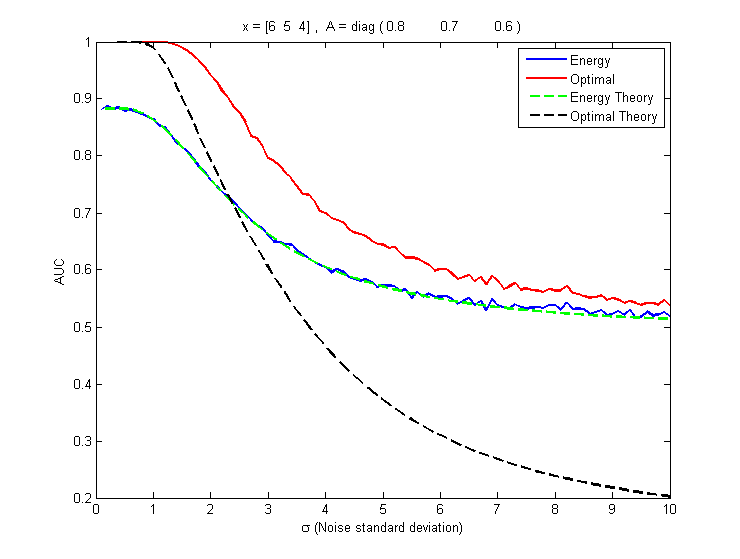
\includegraphics[width=5in]{with_theory.png}
\caption{Empirical and Theory AUC of the different classifiers}
\label{fig:theory_1}
\end{figure}

\subsection{Mean Squared Error of ML Estimate}

\begin{figure}[h!]
\centering
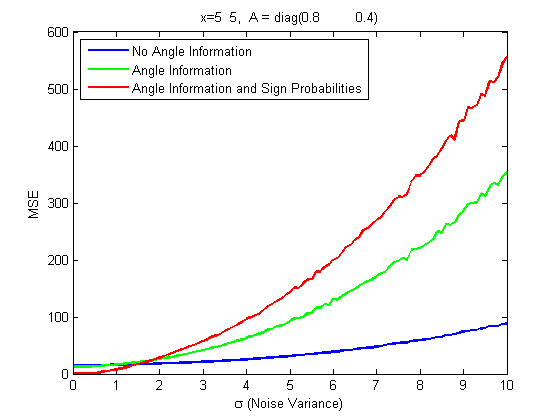
\includegraphics[width=5in]{mse_1.png}
\caption{Empirical MSE of the different classifiers}
\label{fig:mse_1}
\end{figure}

\begin{figure}[h!]
\centering
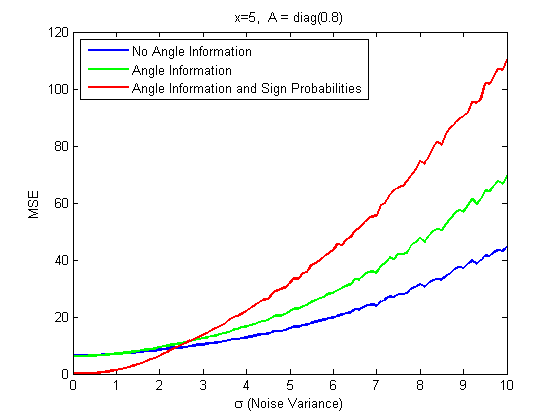
\includegraphics[width=5in]{mse_2.png}
\caption{Empirical MSE of the different classifiers}
\label{fig:mse_2}
\end{figure}

\begin{figure}[h!]
\centering
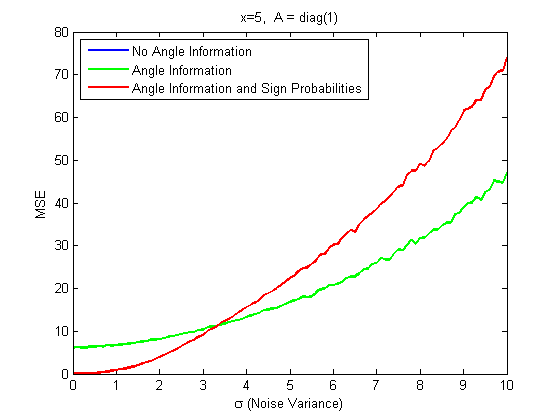
\includegraphics[width=5in]{mse_3.png}
\caption{Empirical MSE of the different classifiers}
\label{fig:mse_3}
\end{figure}

\begin{figure}[h!]
\centering
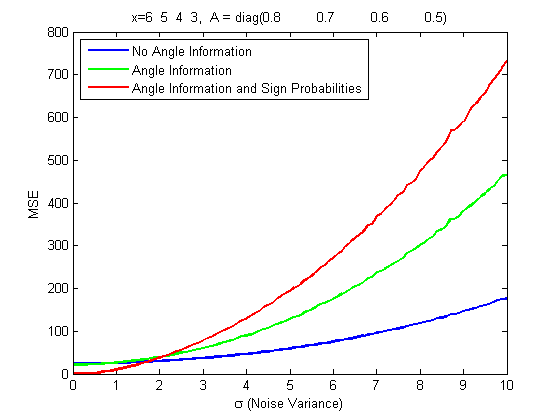
\includegraphics[width=5in]{mse_4.png}
\caption{Empirical MSE of the different classifiers}
\label{fig:mse_4}
\end{figure}

\subsection{AUC Results}

\begin{figure}[h!]
\centering
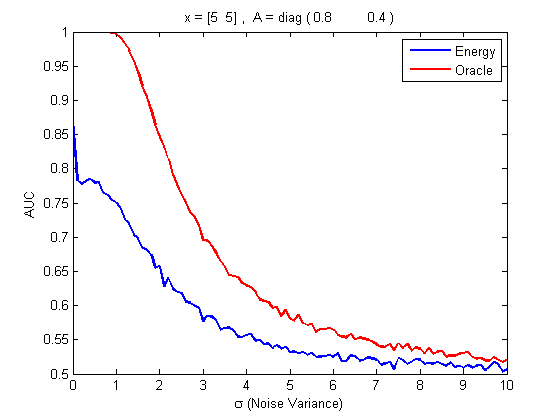
\includegraphics[width=5in]{auc_1.png}
\caption{Empirical AUC of the different classifiers}
\label{fig:auc_1}
\end{figure}

\begin{figure}[h!]
\centering
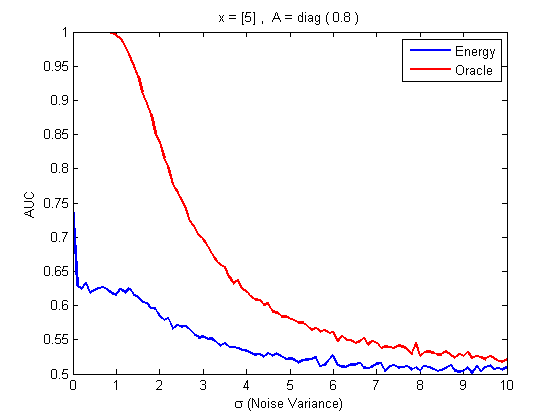
\includegraphics[width=5in]{auc_2.png}
\caption{Empirical AUC of the different classifiers}
\label{fig:auc_2}
\end{figure}

\begin{figure}[h!]
\centering
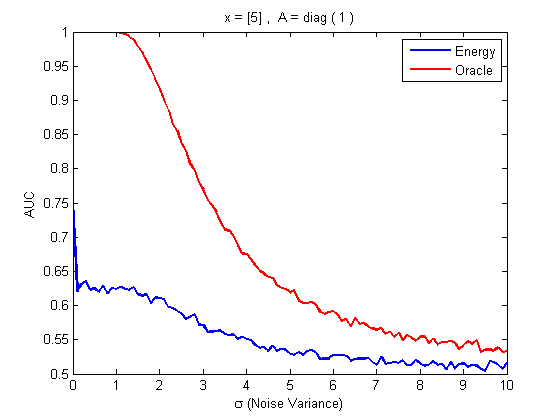
\includegraphics[width=5in]{auc_3.png}
\caption{Empirical AUC of the different classifiers}
\label{fig:auc_3}
\end{figure}

\begin{figure}[h!]
\centering
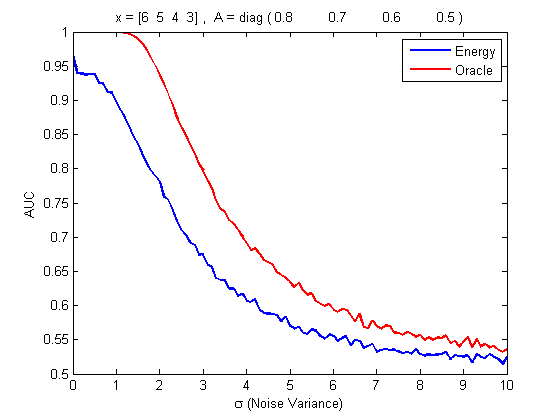
\includegraphics[width=5in]{auc_4.png}
\caption{Empirical AUC of the different classifiers}
\label{fig:auc_4}
\end{figure}

\end{document} 